\documentclass[11pt]{article}

\usepackage{hyperref}
\usepackage{mathtools}
\usepackage{amsthm}
\usepackage{amssymb}
\usepackage{MnSymbol}
\usepackage{mathrsfs}
\usepackage[arrow]{xy}
\usepackage{dsfont}
\usepackage{enumitem}
\usepackage{accents}
\usepackage{tabu}

\pagestyle{headings}

\newcommand{\Z}{\mathbb{Z}}

\theoremstyle{definition}
\newtheorem*{defn}{Definition}

\theoremstyle{definition}
\newtheorem{ex}{Example}

\theoremstyle{plain}
\newtheorem{theo}{Theorem}

\theoremstyle{plain}
\newtheorem{prop}{Proposition}

\theoremstyle{plain}
\newtheorem{lem}{Lemma}

\theoremstyle{definition}
\newtheorem{que}{Question}

\theoremstyle{definition}
\newtheorem{rem}[prop]{Remark}

\begin{document}

\author{Stephen Liu}
\title{Post-Thesis Notes}
\date{April 8, 2020}

\maketitle

\begin{prop}\label{prop:partialres}
Let $d = 2m+1$ be odd and $B_2^d$ be the closed $d$-dimensional Euclidean ball. Then
\begin{equation}\label{eqn:partialres}
\begin{aligned}
&\frac{d^2}{dt^2}\text{Mag}(tB_2^d)\big\vert_{t=0} = \\
&6\sum\limits_{\substack{2\leq p_2\leq m+1 \\ 0\leq q_1 \leq p_2-2 \\ 0\leq q_2 \leq m+1-p_2}}\frac{1}{2p_2-1}\left(\prod\limits_{k=2}^{q_1+1}\frac{(2k-2)}{(2k-1)}\right)\left(\prod\limits_{k=p_2+1}^{p_2+q_2}\frac{(2k-2)}{(2k-1)}\right) + \\
&6\sum\limits_{\substack{2\leq p_1\leq m-1 \\ 0\leq q_1\leq m-1-p_1}}\frac{1}{2p_1-1}\left(\prod\limits_{k=p_1+1}^{p_1+q_1}\frac{(2k-2)}{(2k-1)}\right)\left(\frac{2m}{(2m-1)(2m+1)}\right) + \\
&6\sum\limits_{\substack{2\leq p_1\leq m \\ 0\leq q_1\leq m-p_1}}\frac{1}{2p_1-1}\left(\prod\limits_{k=p_1+1}^{p_1+q_1}\frac{(2k-2)}{(2k-1)}\right)\left(\frac{1}{2m+1}\right) + \\
&6\sum\limits_{\substack{2\leq p_1\leq m \\ p_1+1\leq p_2 \leq m-1 \\ 0\leq q_1\leq p_2-p_1-1 }}\frac{1}{2p_1-1}\left(\prod\limits_{k=p_1+1}^{p_1+q_1}\frac{(2k-2)}{(2k-1)}\right)\frac{1}{2p_2-1}\left(\prod\limits_{k=p_2+1}^{m+1}\frac{(2k-2)}{(2k-1)}\right) - \\
&V_{1}\sum\limits_{\substack{1\leq p \leq m-1 \\ 0 \leq q \leq m - 1 - p}}\frac{1}{2p+1}\prod\limits_{k=p+1}^{p+q}\left(\frac{2k}{2k+1}\right).
\end{aligned}
\end{equation}
where $V_1 = V_1\left(B_2^d\right)$ denotes the first intrinsic volume of $B_2^d$.
\end{prop}

In these notes we will endeavor to simplify the complicated sum given in Proposition (\ref{prop:partialres}) above.

\subsection*{A Different Expression for $V_1$}

Before continuing, we first obtain a different expression for $V_1$ that we will use later. Recall that in terms of the Gamma function, the first intrinsic volume is given by
\begin{equation}\label{eqn:v1gamma}
V_1(B_2^d) = \frac{(2m+1)\sqrt{\pi}\Gamma(m+1)}{\Gamma\left(m+\frac{3}{2}\right)}.
\end{equation}

Recall also that the Legendre Duplication Formula \cite{weisstein_legendre_nodate} is given by

\begin{equation*}
\Gamma\left(z+\frac{1}{2}\right) = \frac{\sqrt{\pi}\Gamma(2z)}{2^{2z-1}\Gamma(z)}.
\end{equation*}

Then for $z = m+1$, we have
\begin{equation}\label{eqn:threehalves}
\Gamma\left(m+\frac{3}{2}\right) = \frac{(2m+1)\sqrt{\pi}\Gamma(2m+1)}{2^{2m+1}\Gamma(m+1)}
\end{equation}

and so we can rewrite (\ref{eqn:v1gamma})
\begin{equation}\label{eqn:v1simp}
\begin{aligned}
V_1(B_2^d) &= \frac{(2m+1)\sqrt{\pi}\Gamma(m+1)}{\Gamma\left(m+\frac{3}{2}\right)} \\
&= \frac{(2m+1)\sqrt{\pi}\Gamma(m+1)\Gamma(m+1)2^{2m+1}}{(2m+1)\sqrt{\pi}\Gamma(2m+1)} \\
&= \frac{2^{2m+1}\Gamma(m+1)^2}{\Gamma(2m+1)} \\
&= \frac{2\cdot2^{2m}(m!)^2}{(2m)!}
\end{aligned}
\end{equation}
where the last equality is because $m$, and therefore $m+1$ and $2m+1$, is an integer.

\subsection*{Skip Factorials}

This section describes ongoing work to further simplify the expression arrived at in Proposition \ref{prop:partialres}. The products
\begin{align}
&\prod\limits_{k=a}^{b}\frac{(2k-2)}{(2k-1)}, \label{eqn:Nskipfact}\\
&\prod\limits_{k=a}^b\frac{2k}{2k+1} \label{eqn:Dskipfact}
\end{align}
that appear in the sums in ({\ref{eqn:partialres}) above are ratios of skip or double factorials. In the following, we will use the identities about skip factorials given below \cite{weisstein_double_nodate}:
\begin{align*}
&(2n)!! = 2^nn!, \\
&(2n-1)!! = \frac{(2n)!}{2^nn!}, \\
&(2n+1)!! = \frac{(2n+1)!}{2^nn!}.
\end{align*}
We will also use Catalan numbers \cite{weisstein_catalan_nodate}, which are defined by
\begin{equation*}
C_n = \frac{1}{n+1}\binom{(2n)}{n} = \frac{1}{2n+1}\binom{(2n+1)}{n}.
\end{equation*}
Using these identities, we rewrite the product (\ref{eqn:Nskipfact}):
\begin{equation}\label{eqn:Nskipfactsimp}
\begin{aligned}
\prod\limits_{k=a}^{b}\frac{(2k-2)}{(2k-1)} &= \frac{2(a-1)}{2a-1}\cdots\frac{2(b-1)}{2b-1} = \frac{(2(b-1))!!}{(2(a-2))!!}\left[\frac{(2b-1)!!}{(2(a-1)-1)!!}\right]^{-1} \\
&= \frac{2^{b-1}(b-1)!}{2^{a-2}(a-2)!}\left[\frac{(2b)!}{2^bb!}\frac{2^{a-1}(a-1)!}{(2(a-1))!}\right]^{-1} \\
&= \frac{2^{2b-1}}{2^{2(a-1)-1}}\frac{b!(b-1)!}{(2b)!}\frac{(2(a-1))!}{(a-1)!(a-2)!} = \frac{2^{2b-1}}{2^{2(a-1)-1}}\frac{(a-1)\binom{2(a-1)}{a-1}}{b\binom{2b}{b}} \\
&= \frac{2^{2b-1}}{2^{2(a-1)-1}}\frac{(a-1)aC_{a-1}}{b(b+1)C_b}.
\end{aligned}
\end{equation}
And similarly we rewrite (\ref{eqn:Dskipfact}):
\begin{equation}\label{eqn:Dskipfactsimp}
\begin{aligned}
\prod\limits_{k=a}^b\frac{2k}{2k+1} &= \frac{2a}{2a+1}\cdots\frac{2b}{2b+1} = \frac{(2b)!!}{(2(a-1))!!}\left[\frac{(2b+1)!!}{(2a-1)!!}\right]^{-1} \\
&= \frac{2^bb!}{2^{a-1}(a-1)!}\left[\frac{(2b+1)!}{2^bb!}\frac{2^aa!}{(2a)!}\right]^{-1} = \frac{2^{2b}}{2^{2a-1}}\frac{(b!)^2}{(2b+1)!}\frac{(2a)!}{a!(a-1)!} \\
&= \frac{2^{2b}}{2^{2a-1}}\frac{a\binom{2a}{a}}{(b+1)\binom{2b+1}{b}} = \frac{2^{2b}}{2^{2a-1}}\frac{a(a+1)C_a}{(2b+1)(b+1)C_b}.
\end{aligned}
\end{equation}

\begin{rem}
Here is our general approach to simplifying sums in (\ref{eqn:partialres}):
\begin{enumerate}[label=\arabic*.]
\item Use (\ref{eqn:Nskipfactsimp}) or (\ref{eqn:Dskipfactsimp}) to simplify the products appearing in the sum.
\item Employ the change of variables $k = p+q$ and summing over $k$ and $p$ to rewrite the result of step 1 above into a sum over $k$ multiplied by a sum over $p$ (where the top bound is dependent on $k$).
\item Use Wolfram Alpha to get a simple expression for the inner sum (the sum over $p$).
\item Substitute the result gotten above into the sum over $k$ and use Wolfram Alpha again to simplify.
\end{enumerate}
\end{rem}

\subsubsection*{The last sum in (\ref{eqn:partialres})}

We will first try to simplify the very last sum in (\ref{eqn:partialres}). Using (\ref{eqn:Dskipfactsimp}), we can rewrite the last sum in (\ref{eqn:partialres}) as the following:
\begin{align*}
&V_{1}\sum\limits_{\substack{1\leq p \leq m-1 \\ 0 \leq q \leq m - 1 - p}}\frac{1}{2p+1}\prod\limits_{k=p+1}^{p+q}\left(\frac{2k}{2k+1}\right) \\
&\qquad= V_1\sum\limits_{\substack{1\leq p \leq m-1 \\ 0 \leq q \leq m-1-p}} \frac{1}{2p+1}\frac{2^{2(p+q)}}{2^{2(p+1)-1}}\frac{(p+1)(p+2)C_{p+1}}{(2(p+q)+1)(p+q+1)C_{p+q}}.
\end{align*}
Setting $k = p+q$, this last sum turns into
\begin{equation}
\begin{aligned}\label{eqn:lastvarchange}
&V_1\sum\limits_{k=1}^{m-1}\sum\limits_{p=1}^k\frac{1}{2p+1}\frac{2^{2k}}{2^{2(p+1)-1}}\frac{(p+1)(p+2)C_{p+1}}{(2k+1)(k+1)C_k} \\
&\qquad= V_1\sum\limits_{k=1}^{m-1}\frac{2^{2k}}{(2k+1)(k+1)C_k}\sum\limits_{p=1}^k\frac{(p+1)(p+2)C_{p+1}}{2^{2p+1}(2p+1)}.
\end{aligned}
\end{equation}

The inner sum on the right hand side of the above can be further simplified
\begin{equation}\label{eqn:lastinnersum}
\begin{aligned}
\sum\limits_{p=1}^k\frac{(p+1)(p+2)C_{p+1}}{2^{2p+1}(2p+1)} &= \sum\limits_{p=1}^k\frac{(p+1)(p+2)\frac{1}{p+2}\binom{2(p+1)}{p+1}}{2^{2p+1}(2p+1)} \\
&= \sum\limits_{p=1}^k\frac{(p+1)\frac{(2(p+1))!}{[(p+1)!]^2}}{2^{2p+1}(2p+1)} \\
&= \sum\limits_{p=1}^k\frac{(2(p+1))!}{p!(p+1)!2^{2p+1}(2p+1)}.
\end{aligned}
\end{equation}

Wolfram Alpha says that the last sum of (\ref{eqn:lastinnersum}) can be simplified to
\begin{equation}\label{eqn:lastinnersum2}
\sum\limits_{p=1}^k\frac{(2(p+1))!}{p!(p+1)!2^{2p+1}(2p+1)} = \frac{(k+1)(2(k+2))!}{2^{2(k+1)}(2k+3)(k+1)!(k+2)!}-1.
\end{equation}

So substituting the right hand side of (\ref{eqn:lastinnersum2}) into (\ref{eqn:lastvarchange}) above we have
\begin{equation}\label{eqn:simplifiedlast2}
\begin{aligned}
&V_1\sum\limits_{k=1}^{m-1}\frac{2^{2k}}{(2k+1)(k+1)C_k}\sum\limits_{p=1}^k\frac{(p+1)(p+2)C_{p+1}}{2^{2p+1}(2p+1)} \\
&\quad=V_1\sum\limits_{k=1}^{m-1}\frac{2^{2k}}{(2k+1)(k+1)C_k}\left[\frac{(k+1)(2(k+2))!}{2^{2(k+1)}(2k+3)(k+1)!(k+2)!}-1\right] \\
&= V_1\left[\sum\limits_{k=1}^{m-1}\frac{2^{2k}}{(2k+1)(k+1)C_k}\cdot\frac{(k+1)(2(k+2))!}{2^{2(k+1)}(2k+3)(k+1)!(k+2)!}\right. \\
&\qquad - \left.\sum\limits_{k=1}^{m-1}\frac{2^{2k}}{(2k+1)(k+1)C_k}\right]
\end{aligned}
\end{equation}

Plugging in the definition of $C_k$, the second sum in (\ref{eqn:simplifiedlast2}) simplifies to:
\begin{equation}\label{eqn:lastsecond}
\begin{aligned}
\sum\limits_{k=1}^{m-1}\frac{2^{2k}}{(2k+1)(k+1)C_k} &= \sum\limits_{k=1}^{m-1}\frac{2^{2k}(k+1)[k!]^2}{(2k+1)(k+1)(2k)!} \\
&= \sum\limits_{k=1}^{m-1}\frac{2^{2k}[k!]^2}{(2k+1)(2k)!} \\
&= \frac{2^{2m}[m!]^2}{(2m)!}-2 \\
&= \frac{1}{2}V_1 - 2.
\end{aligned}
\end{equation}
where the second to last equality is given by Wolfram Alpha and the last equality is by (\ref{eqn:v1simp}).

The first sum in (\ref{eqn:simplifiedlast2}) simplifies to:
\begin{equation}\label{eqn:lastfirst}
\begin{aligned}
&\sum\limits_{k=1}^{m-1}\frac{2^{2k}}{(2k+1)(k+1)C_k}\frac{(k+1)(2(k+2))!}{2^{2(k+1)}(2k+3)(k+1)!(k+2)!} \\
&\quad= \sum\limits_{k=1}^{m-1}\frac{2^{2k}}{2^{2(k+1)}}\frac{(k+1)^2(2(k+2))![k!]^2}{(2k+1)(k+1)(2k+3)(k+1)!(k+2)!(2k)!} \\
&\quad= \sum\limits_{k=1}^{m-1}\frac{1}{2^2}\frac{(k+1)(2(k+2))![k!]^2}{(2k+1)(2k+3)(k+1)!(k+2)!(2k)!} \\
&\quad= \sum\limits_{k=1}^{m-1}\frac{1}{2^2}\frac{(2(k+2))![k!]^2}{(2k+1)(2k+3)k!(k+2)!(2k)!} \\
&\quad= \sum\limits_{k=1}^{m-1}\frac{1}{2^2}\frac{(2(k+2))!k!}{(2k+1)(2k+3)(k+2)!(2k)!} \\
&\quad = \sum\limits_{k=1}^{m-1}\frac{1}{2^2}\frac{(2(k+2))!}{(2k+1)(2k+3)(k+1)(k+2)(2k)!} \\
&\quad = \sum\limits_{k=1}^{m-1}\frac{1}{2^2}\frac{(2k+1)(2k+2)(2k+3)(2k+4)}{(2k+1)(2k+3)(k+1)(k+2)} \\
&\quad = \sum\limits_{k=1}^{m-1}\frac{1}{2^2}\frac{(2k+2)(2k+4)}{(k+1)(k+2)} \\
&\quad = \sum\limits_{k=1}^{m-1}\frac{1}{2^2}\frac{2(k+1)2(k+2)}{(k+1)(k+2)} \\
&\quad = m-1.
\end{aligned}
\end{equation}

So putting (\ref{eqn:lastfirst}) and (\ref{eqn:lastsecond}) together we have
\begin{equation}\label{eqn:lastsimp}
\begin{aligned}
V_1\sum\limits_{\substack{1\leq p \leq m -1 \\ 0 \leq q \leq m-1-p}}\frac{1}{2p+1}\prod\limits_{k=p+1}^{p+q}\left(\frac{2k}{2k+1}\right) = V_1\left(m+1 - \frac{1}{2}V_1\right) = -\frac{1}{2}V_1^2+V_1(m+1).
\end{aligned}
\end{equation}

\subsubsection*{The second and third sum in (\ref{eqn:partialres})}

We employ a similar process to simplify the other double sums that appear in (\ref{eqn:partialres}). We first simplify
\begin{equation}\label{eqn:third}
6\sum\limits_{\substack{2 \leq p \leq m \\ 0 \leq q \leq m - p}} \frac{1}{2p-1}\left(\prod\limits_{k=p+1}^{p+q}\frac{(2k-2)}{(2k-1)}\right)\left(\frac{1}{2m+1}\right).
\end{equation}

Here, we've dropped the subscripts on the variables $p_1$ and $q_1$ for convenience. We can factor out $\frac{1}{2m+1}$ first, so we'll disregard it, along with the 6 on the outside, in our calculations below. Using (\ref{eqn:Nskipfactsimp}), we have that (\ref{eqn:third}) (without the $\frac{1}{2m+1}$ term) is equal to
\begin{equation}\label{eqn:thirdsimplified1}
\sum\limits_{\substack{2\leq p \leq m \\ 0 \leq q \leq m-p}} \frac{1}{2p-1}\frac{2^{2(p+q)-1}}{2^{2p-1}}\frac{p(p+1)C_p}{(p+q)(p+q+1)C_{p+q}}.
\end{equation}

Setting $k = p + q$, (\ref{eqn:thirdsimplified1}) becomes
\begin{equation}\label{eqn:thirdvarchange}
\begin{aligned}
&\sum\limits_{\substack{2\leq p \leq m \\ 0 \leq q \leq m-p}} \frac{1}{2p-1}\frac{2^{2(p+q)-1}}{2^{2p-1}}\frac{p(p+1)C_p}{(p+q)(p+q+1)C_{p+q}} \\
&\qquad= \sum\limits_{k=2}^m\sum\limits_{p=2}^k \frac{1}{2p-1}\frac{2^{2k-1}}{2^{2p-1}}\frac{p(p+1)C_p}{k(k+1)C_k} \\
&\qquad= \sum\limits_{k=2}^m\frac{2^{2k-1}}{k(k+1)C_k}\sum\limits_{p=2}^k\frac{p(p+1)C_p}{2^{2p-1}(2p-1)}
\end{aligned}
\end{equation}

Plugging in the definition of $C_p$, the sum over $p$ in (\ref{eqn:thirdvarchange}) simplifies to
\begin{equation}\label{eqn:thirdinnersum}
\begin{aligned}
\sum\limits_{p=2}^k\frac{p(p+1)C_p}{2^{2p-1}(2p-1)} &= \sum\limits_{p=2}^k\frac{p(p+1)\frac{1}{p+1}\frac{(2p)!}{[p!]^2}}{2^{2p-1}(2p-1)} \\
&= \sum\limits_{p=2}^k\frac{p(2p)!}{2^{2p-1}(2p-1)[p!]^2} \\
&= \sum\limits_{p=2}^k\frac{(2p)!}{2^{2p-1}(2p-1)p!(p-1)!} \\
&= \frac{k(2(k+1))!}{2^{2k}(2k+1)k!(k+1)!}-1,
\end{aligned}
\end{equation}

where the last equality is given by Wolfram Alpha. Simplifying the sum over $k$ in (\ref{eqn:thirdvarchange}), we have
\begin{equation}\label{eqn:thirdoutersum}
\begin{aligned}
\sum\limits_{k=2}^m\frac{2^{2k-1}}{k(k+1)C_k} &= \sum\limits_{k=2}^m\frac{2^{2k-1}}{k(k+1)\frac{1}{k+1}\frac{(2k)!}{[k!]^2}} \\
&= \sum\limits_{k=2}^m \frac{2^{2k-1}[k!]^2}{k(2k)!} \\
&= \frac{2^{2m+1}(2m+1)((m+1)!)^2}{(m+1)(2m+2)!}-2 \\
&= \frac{2^{2m+1}(2m+1)(m+1)^2(m!)^2}{2(m+1)^2(2m+1)(2m)!} - 2 \\
&= \frac{2^{2m+1}(m!)^2}{2(2m)!}-2 \\
&= \frac{1}{2}V_1 - 2.
\end{aligned}
\end{equation}

Then plugging in (\ref{eqn:thirdinnersum}) and (\ref{eqn:thirdoutersum}) into (\ref{eqn:thirdvarchange}) above, we have

\begin{equation}
\begin{aligned}
&\sum\limits_{k=2}^m\frac{2^{2k-1}}{k(k+1)C_k}\sum\limits_{p=2}^k\frac{p(p+1)C_p}{2^{2p-1}(2p-1)} \\
&\qquad = \sum\limits_{k=2}^m\frac{2^{2k-1}[k!]^2}{k(2k)!}\frac{k(2(k+1))!}{2^{2k}(2k+1)k!(k+1)!} - \left[\frac{1}{2}V_1-2\right] \\
&\qquad = \sum\limits_{k=2}^m\frac{2^{2k-1}}{2^{2k}}\frac{[k!]^2k(2(k+1))!}{k(2k)!(2k+1)k!(k+1)!} - \frac{1}{2}V_1 + 2 \\
&\qquad = \sum\limits_{k=2}^m \frac{1}{2}\frac{k!}{(k+1)!}\frac{(2k+1)(2k+2)}{(2k+1)} -\frac{1}{2}V_1 + 2 \\
&\qquad = \sum\limits_{k=2}^m \frac{1}{2}\frac{(2k+2)}{(k+1)} - \frac{1}{2}V_1 + 2 \\
&\qquad = \sum\limits_{k=2}^m \frac{1}{2}\frac{2(k+1)}{(k+1)}  - \frac{1}{2}V_1 + 2 \\
&\qquad = m - 1 - \frac{1}{2}V_1 + 2 \\
&\qquad = m + 1 - \frac{1}{2}V_1.
\end{aligned}
\end{equation}

So we have that 
\begin{equation}\label{eqn:thirdsimp}
\begin{aligned}
6\sum\limits_{\substack{2 \leq p \leq m \\ 0 \leq q \leq m - p}} \frac{1}{2p-1}\left(\prod\limits_{k=p+1}^{p+q}\frac{(2k-2)}{(2k-1)}\right)\left(\frac{1}{2m+1}\right) &= \frac{6}{2m+1}\left(m + 1 - \frac{1}{2}V_1\right) \\
&= \frac{6(m+1)}{2m+1} - \frac{3V_1}{2m+1}
\end{aligned}
\end{equation}

Applying the same process to the second sum in (\ref{eqn:partialres}), we have
\begin{equation}\label{eqn:secondsimp}
\begin{aligned}
&6\sum\limits_{\substack{2\leq p \leq m -1 \\ 0 \leq q \leq m - 1 - p}}\frac{1}{2p-1}\left(\prod\limits_{k=p+1}^{p+q}\frac{(2k-2)}{(2k-1)}\right)\left(\frac{2m}{(2m-1)(2m+1)}\right) \\
&\qquad = \frac{12m^2}{(2m-1)(2m+1)} - \frac{3V_1}{2m+1}.
\end{aligned}
\end{equation}

\subsection*{The first sum in (\ref{eqn:partialres})}

We now simplify the first sum in (\ref{eqn:partialres}), that is, the sum
\begin{equation}\label{eqn:first}
\sum\limits_{p_2=2}^{m+1}\sum\limits_{q_1=0}^{p_2-2}\sum\limits_{q_2=0}^{m+1-p_2}\frac{1}{2p_2-1}\left(\prod\limits_{k=2}^{q_1+1}\frac{(2k-2)}{(2k-1)}\right)\left(\prod\limits_{k=p_2+1}^{p_2+q_2}\frac{(2k-2)}{(2k-1)}\right).
\end{equation}

First we use (\ref{eqn:Nskipfactsimp}) to simplify the products in the sum above. We have
\begin{equation}\label{eqn:firstprod1}
\begin{aligned}
\prod\limits_{k=2}^{q_1+1}\frac{(2k-2)}{(2k-1)} &= \frac{2^{2(q_1+1)-1}}{2^{2(2-1)-1}}\frac{(2-1)2C_{2-1}}{(q_1+1)(q_1+2)C_{q_1+1}} \\
&= \frac{2^{2(q_1+1)-1}}{2}\frac{2C_{1}}{(q_1+1)(q_1+2)C_{q_1+1}} \\
&= \frac{2^{2(q_1+1)-1}}{(q_1+1)(q_1+2)C_{q_1+1}}
\end{aligned}
\end{equation}
and
\begin{equation}\label{eqn:firstprod2}
\prod\limits_{k=p_2+1}^{p_2+q_2}\frac{(2k-2)}{(2k-1)} = \frac{2^{2(p_2+q_2)-1}}{2^{2p_2-1}}\frac{p_2(p_2+1)C_{p_2}}{(p_2+q_2)(p_2+q_2+1)C_{p_2+q_2}}
\end{equation}

Substituting (\ref{eqn:firstprod1}) and (\ref{eqn:firstprod2}) into (\ref{eqn:first}) and employing the change of variables $k = p_2+q_2$ and $\ell = q_1+1$, we have
\begin{equation}\label{eqn:firstseparated}
\begin{aligned}
&\sum\limits_{p_2=2}^{m+1}\sum\limits_{q_1=0}^{p_2-2}\sum\limits_{q_2=0}^{m+1-p_2}\frac{1}{2p_2-1}\left(\prod\limits_{k=2}^{q_1+1}\frac{(2k-2)}{(2k-1)}\right)\left(\prod\limits_{k=p_2+1}^{p_2+q_2}\frac{(2k-2)}{(2k-1)}\right)\\
&\quad = \sum\limits_{p_2=2}^{m+1}\sum\limits_{q_1=0}^{p_2-2}\sum\limits_{q_2=0}^{m+1-p_2}\frac{1}{2p_2-1}\frac{2^{2(q_1+1)-1}}{(q_1+1)(q_1+2)C_{q_1+1}}\frac{2^{2(p_2+q_2)-1}}{2^{2p_2-1}}\frac{p_2(p_2+1)C_{p_2}}{(p_2+q_2)(p_2+q_2+1)C_{p_2+q_2}} \\
&\quad = \sum\limits_{k=2}^{m+1}\frac{2^{2k-1}}{k(k+1)C_k}\sum\limits_{p_2=2}^k\frac{p_2(p_2+1)C_{p_2}}{(2p_2-1)2^{2p_2-1}}\sum\limits_{\ell=1}^{p_2-1}\frac{2^{2\ell-1}}{\ell(\ell+1)C_\ell}.
\end{aligned}
\end{equation}

Now we just simplify from the innermost sum out. With help from Wolfram Alpha, we have that the innermost sum in (\ref{eqn:firstseparated}) simplifies to:

\begin{equation}\label{eqn:firstinnermost}
\begin{aligned}
\sum\limits_{\ell=1}^{p_2-1}\frac{2^{2\ell-1}}{\ell(\ell+1)C_\ell} &= \sum\limits_{\ell = 1}^{p_2-1} \frac{2^{2\ell-1}(\ell!)^2}{\ell(2\ell)!} \\
&= \frac{2^{2p_2-1}(2p_2-1)(p_2!)^2}{p_2(2p_2)!} - 1 \\
&= \frac{2^{2p_2-1}(2p_2-1)}{p_2(p_2+1)C_{p_2}} - 1.
\end{aligned}
\end{equation}

Then substituting (\ref{eqn:firstinnermost}) into the second innersum of (\ref{eqn:firstseparated}), we have

\begin{equation}\label{eqn:firstsecondinner}
\begin{aligned}
\sum\limits_{p_2=2}^k\frac{p_2(p_2+1)C_{p_2}}{(2p_2-1)2^{2p_2-1}}\sum\limits_{\ell=1}^{p_2-1}\frac{2^{2\ell-1}}{\ell(\ell+1)C_\ell} &= \sum\limits_{p_2=2}^k\frac{p_2(p_2+1)C_{p_2}}{(2p_2-1)2^{2p_2-1}}\left[\frac{2^{2p_2-1}(2p_2-1)}{p_2(p_2+1)C_{p_2}} - 1\right] \\
&= \sum\limits_{p_2=2}^k\frac{p_2(p_2+1)C_{p_2}}{(2p_2-1)2^{2p_2-1}}\frac{2^{2p_2-1}(2p_2-1)}{p_2(p_2+1)C_{p_2}} - \sum\limits_{p_2=2}^k\frac{p_2(p_2+1)C_{p_2}}{(2p_2-1)2^{2p_2-1}} \\
&= (k-1) - \sum\limits_{p_2=2}^k\frac{p_2(p_2+1)C_{p_2}}{(2p_2-1)2^{2p_2-1}} \\
&= (k-1) - \left[\frac{k(k+1)(2(k+1))!}{2^{2k}(2k+1)((k+1)!)^2}-1\right] \\
&= k - \frac{k(k+1)(2(k+1))!}{2^{2k}(2k+1)((k+1)!)^2}
\end{aligned}
\end{equation}
where the second last equality is again via Wolfram Alpha/Mathematica.

Finally, substituting (\ref{eqn:firstsecondinner}) into (\ref{eqn:firstseparated}) and simplifying, we have

\begin{equation}\label{eqn:firstsimplified}
\begin{aligned}
&\sum\limits_{k=2}^{m+1}\frac{2^{2k-1}}{k(k+1)C_k}\sum\limits_{p_2=2}^k\frac{p_2(p_2+1)C_{p_2}}{(2p_2-1)2^{2p_2-1}}\sum\limits_{\ell=1}^{p_2-1}\frac{2^{2\ell-1}}{\ell(\ell+1)C_\ell} \\
&\quad= \sum\limits_{k=2}^{m+1}\frac{2^{2k-1}}{k(k+1)C_k}\left[k - \frac{k(k+1)(2(k+1))!}{2^{2k}(2k+1)((k+1)!)^2}\right] \\
&\quad = \sum\limits_{k=2}^{m+1}\frac{2^{2k-1}}{(k+1)C_k} - \sum\limits_{k=2}^{m+1}\frac{2^{2k-1}}{k(k+1)C_k}\frac{k(k+1)(2(k+1))!}{2^{2k}(2k+1)((k+1)!)^2} \\
&\quad = \sum\limits_{k=2}^{m+1}\frac{2^{2k-1}}{(k+1)C_k} - \sum\limits_{k=2}^{m+1}\frac{1}{2}\frac{k(k+1)(2(k+1))!(k+1)(k!)^2}{k(k+1)(2k)!(2k+1)((k+1)!)^2} \\
&\quad = \sum\limits_{k=2}^{m+1}\frac{2^{2k-1}}{(k+1)C_k} - \sum\limits_{k=2}^{m+1}\frac{1}{2}\frac{(2k+1)(2k+2)(2k)!(k+1)(k!)^2}{(2k)!(2k+1)((k+1)!)^2} \\
&\quad = \sum\limits_{k=2}^{m+1}\frac{2^{2k-1}}{(k+1)C_k} - \sum\limits_{k=2}^{m+1}\frac{1}{2}\frac{(2k+1)}{(k+1)} \\
&\quad = \sum\limits_{k=2}^{m+1}\frac{2^{2k-1}}{(k+1)C_k} - m \\
&\quad = \frac{1}{3}\left[\frac{\sqrt{\pi}\Gamma(m+3)}{\Gamma\left(m+\frac{3}{2}\right)}-4\right] - m \\
&\quad = \frac{\sqrt{\pi}(m+2)(m+1)(2m+1)\Gamma(m+1)}{3(2m+1)\Gamma\left(m+\frac{3}{2}\right)} - \frac{4}{3} - m \\
&\quad = \frac{(m+2)(m+1)}{3(2m+1)}V_1-\frac{4}{3}-m
\end{aligned}
\end{equation}
where the identity relating the sum to the Gamma function is from Wolfram Alpha/Mathematica and the last equality is again by (\ref{eqn:v1simp}).

So the first sum in (\ref{eqn:partialres}) simplifies to
\begin{equation}\label{eqn:firstsimp2}
\begin{aligned}
&6\sum\limits_{\substack{2\leq p_2\leq m+1 \\ 0\leq q_1 \leq p_2-2 \\ 0\leq q_2 \leq m+1-p_2}}\frac{1}{2p_2-1}\left(\prod\limits_{k=2}^{q_1+1}\frac{(2k-2)}{(2k-1)}\right)\left(\prod\limits_{k=p_2+1}^{p_2+q_2}\frac{(2k-2)}{(2k-1)}\right) \\
&\qquad = 6\left(\frac{(m+2)(m+1)}{3(2m+1)}V_1-\frac{4}{3}-m\right) \\
&\qquad = \frac{2(m+2)(m+1)}{(2m+1)}V_1-8-6m.
\end{aligned}
\end{equation}

\subsection*{Estimating the Second Order Term}

Unfortunately, due to the way the bounds on the indices in the fourth sum in (\ref{eqn:partialres}) are interrelated, I haven't yet been able to simplify the fourth sum in a similar way as above. However, notice that every factor in each summand in the fourth sum is a positive quantity, so by omitting the fourth sum we can arrive at a lower bound for the second order term. Moreover, for $m = 1,2,3$, there are no collections of Schröder paths that correspond to the case covered by this fourth sum, so in these cases, this lower bound will be exact. That is, we can already arrive at an exact formula for the second order term for dimensions 3, 5 and 7. Unfortunately, as the dimension increases, the collections of Schröder paths represented by the fourth sum become the majority of collections of paths that need to be considered, so this is estimate becomes worse as we take $d \to \infty$ (see Figure (\ref{fig:estimate})).

\begin{figure}[h!]
\centerline{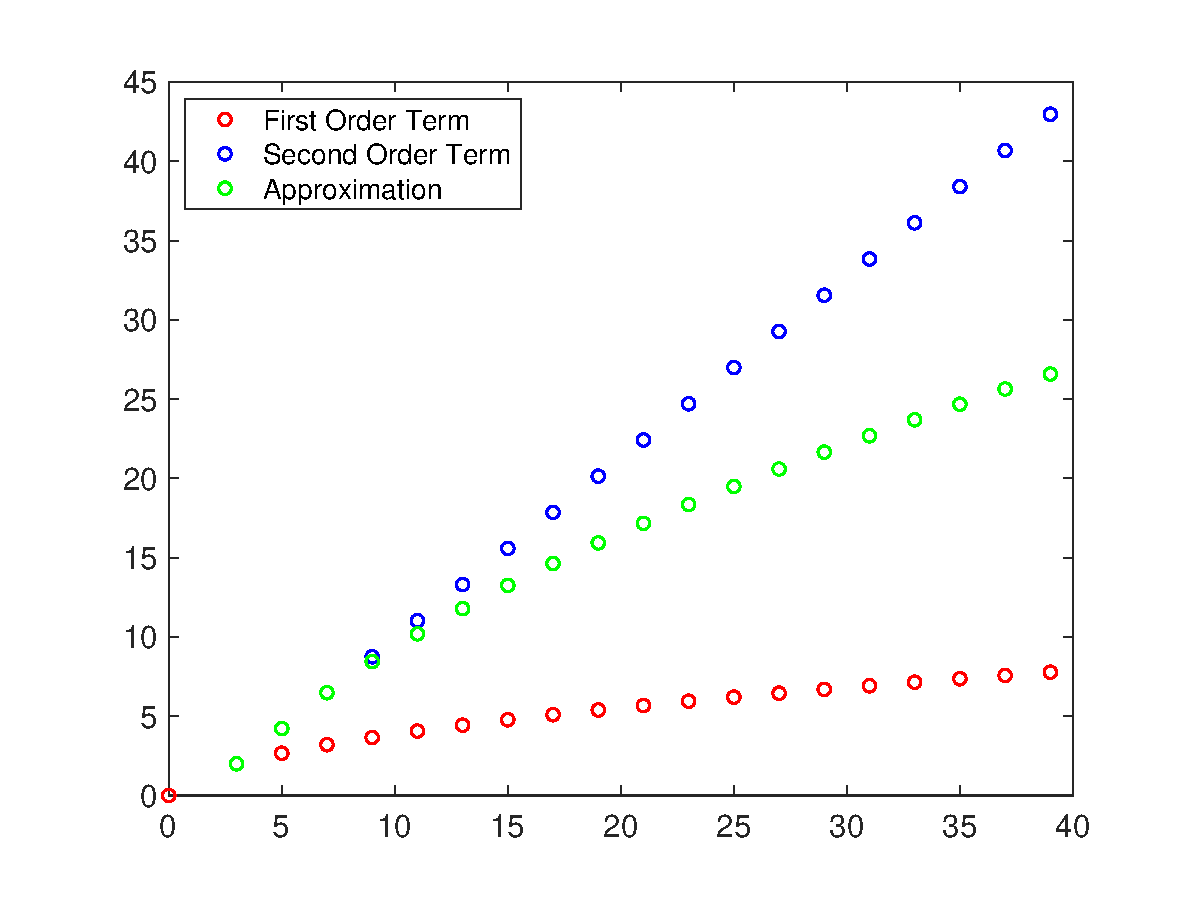
\includegraphics[width=10cm]{estimate.eps}}\caption{\label{fig:estimate} Values of the first order term, the second order term and the estimate for $d = 3$ to 39.}
\end{figure}

Combining (\ref{eqn:firstsimp2}), (\ref{eqn:secondsimp}), (\ref{eqn:thirdsimp}) and (\ref{eqn:lastsimp}) as in (\ref{eqn:partialres}) and simplifying, we arrive at the following result:

\begin{prop}\label{prop:res}
Let $d = 3,5,7$ and $B_2^d$ be the closed $d$-dimensional Euclidean ball. Then
\begin{equation}
\frac{d^2}{dt^2}\text{Mag}\left(tB_2^d\right)\big\vert_{t=0} = \frac{1}{2}V_1^2+V_1\left(\frac{3(m-1)}{2m+1}\right)-\frac{2(12m^3+4m^2-6m-1)}{(2m-1)(2m+1)}.
\end{equation}
\end{prop}

\pagebreak

\bibliographystyle{alpha}
\bibliography{refs.bib}

\end{document}